\documentclass{article}

% Formatting
\usepackage[utf8]{inputenc}
\usepackage[margin=1in]{geometry}
\usepackage[titletoc,title]{appendix}
\usepackage[spanish]{babel}
\usepackage{amsmath,amsfonts,amssymb,mathtools}
\usepackage{graphicx,float}
\usepackage[ruled,vlined]{algorithm2e}
\usepackage{algorithmic}
\usepackage{minted}
\usemintedstyle{borland}
\usepackage{biblatex}

% Title content
\title{Práctica 1 Movimiento Browniano}
\author{Denisse leyva}
\date{Febrero 17, 2021}

\begin{document}

\maketitle

% Introduction
\section{Introducción}
En esta práctica número 1 se trata el tema Movimiento Browniano de una partícula, se debe analizar el tiempo de regreso al origen de dicha partícula en diferentes dimensiones (de 1 a 5) en incrementos lineales, variando el número de pasos de la caminata como potencias de dos con exponente de 4 a 9 en incrementos lineales de uno, con 30 repeticiones del experimento para cada combinación.[1]  


\section{Objetivo}
El objetivo de la simulación es verificar por medio de las 5 dimensiones y las 30 repeticiones en cada cantidad de pasos especifica cuanto se tarda la partícula en regresar al origen o si no regresa nunca. 
Y graficar los datos resultantes en un diagrama caja-bigote, así como obtener un cuadro con la información del mínimo, promedio y máximo del tiempo de regreso para cada dimensión, así como el porcentaje de las que nunca regresaron.



\section{Código}
En el siguiente código se utilizaron secuencias for para realizar todo el objetivo propuesto en una sola ejecución.
Todo está centrado en el primer for que determina la cantidad de pasos. En el segundo for se determina la dimensión a trabajar con el número de pasos que arrojo el for anterior. En el tercer for se especifican las repeticiones para cada dimensión.\\
Además, se utilizó la librería pandas para crear las tablas con el mínimo, promedio, máximo y el porcentaje de las partículas que nunca regresaron al origen.\\
El código base se sacó del repertorio de la Dra. Elisa Schaeffer\\ https://github.com/satuelisa/Simulation/tree/master/BrownianMotion
\\


**Código creado en Python**\\
\begin{verbatim}
from random import random, randint
import matplotlib.pyplot as plt 
import pandas as pd

rff, expt = [], []
for e in range(6):
    exponencial = e + 4
    exp = 2 ** exponencial
    print('Con numero de pasos de ', exp)
    rf=[],[],[],[],[]
    minimo, maximo, promedio, porcentaje = [],[],[],[]
    for d in range(5):
        dimension = d+1
        p_inicial = [0] * dimension
        resultados = []
        resultados1 = []
        repeticiones = 30
    
        for nr in range(repeticiones):
            nunca = True
    
            for paso in range(exp):
                dim = randint(0, dimension-1)
                p_inicial[dim] = p_inicial[dim] + 1 if random() < 0.5 else p_inicial[dim] -1
                
                if all([p == 0 for p in p_inicial]):
                    resultados.append(paso+1)
                    resultados1.append(paso+1)
                    nunca = False
                    break
            if nunca:
                resultados.append(None)
                # resultados1.append(exp+1)
        
        cuantos = sum([r is None for r in resultados])
        # print((cuantos / repeticiones)*100, 'no regresaron nunca en la dimension ', d+1)
        porcentaje.append((cuantos / repeticiones)*100)
        if cuantos < repeticiones:
            regresaron = sum([r if r is not None else 0 for r in resultados])
            # print(regresaron / (repeticiones - cuantos), 'fue la tardanza en promedio en la dimension ', d+1)
        for r in resultados1:
            rf[d].append(r) 
        # print(rf[d])
        if rf[d] > []:
            mi = min(rf[d])
            prom = sum(rf[d])/len(rf[d])
            ma = max(rf[d])
            minimo.append(mi)
            promedio.append(prom)
            maximo.append(ma)
        else:
            # print("se anula")
            minimo.append('Anulado')
            promedio.append('Anulado')
            maximo.append('Anulado')
        
            
    data = {'Dimension':[1,2,3,4,5], 
            'Minimo':minimo, 
            'Promedio':promedio, 
            'Maximo':maximo,
            'Porcentaje':porcentaje} 
    # print(data)
    expt.append(exp)
    rff.append(rf)
    df = pd.DataFrame(data)
    print(df)
        
fig = plt.figure()
gs = fig.add_gridspec(2,3, hspace=0.4, wspace=0.35)
ax1 = fig.add_subplot(gs[0,0])
ax1.boxplot(rff[0])
ax1.set_title('Pasos: ' + str(expt[0]))

ax2 = fig.add_subplot(gs[0,1])
ax2.boxplot(rff[1])
ax2.set_title('Pasos: ' + str(expt[1]))
                      
ax3 = fig.add_subplot(gs[0,2])
ax3.boxplot(rff[2])
ax3.set_title('Pasos: ' + str(expt[2]))

ax4 = fig.add_subplot(gs[1,0])
ax4.boxplot(rff[3])
ax4.set_title('Pasos: ' + str(expt[3]))

ax5 = fig.add_subplot(gs[1,1])
ax5.boxplot(rff[4])
ax5.set_title('Pasos: ' + str(expt[4]))

ax6 = fig.add_subplot(gs[1,2])
ax6.boxplot(rff[5])
ax6.set_title('Pasos: ' + str(expt[5]))

fig.savefig('p1_pasos.png')
# plt.close()
\end{verbatim}
\newpage
% Computational Results
\section{Resultados}
En las Figuras de la 1 a la 6 se muestra un diagrama caja-bigote con los datos de las partículas que regresaron al origen con los pasos determinados en la caminata.

\begin{figure}[H]
\centering
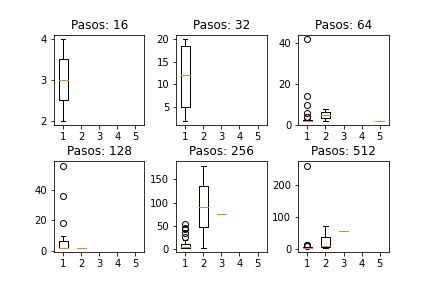
\includegraphics[width=120mm]{p1_pasos.png}
\caption{\label{fig1}Caminata de pasos.}
\end{figure}


En las tablas de la 1 a la 6 se muestran las tablas con el mínimo, el promedio, el máximo y el porcentaje de las partículas que regresaron al origen.\\

\begin{table}[H]
\centering
\begin{tabular}{ |p{2cm}||p{2cm}|p{2cm}|p{2cm}|p{2cm  }|}
 \hline
 \multicolumn{5}{|c|}{Con numero de pasos 16} \\
 \hline
 Dimensión&Minimo&Promedio&Máximo&Porcentaje\\
 \hline
 1   & 2       & 3        & 4       & 93.333333\\
 2   & Anulado & Anulado  & Anulado & 100.000000\\
 3   & Anulado & Anulado  & Anulado & 100.000000\\
 4   & Anulado & Anulado  & Anulado & 100.000000\\
 5   & Anulado & Anulado  & Anulado & 100.000000\\
 \hline
\end{tabular}
\caption{Caminata 16 pasos}
\label{table:1}
\end{table}

\begin{table}[H]
\centering
\begin{tabular}{ |p{2cm}||p{2cm}|p{2cm}|p{2cm}|p{2cm  }|}
 \hline
 \multicolumn{5}{|c|}{Con numero de pasos 32} \\
 \hline
 Dimensión&Minimo&Promedio&Máximo&Porcentaje\\
 \hline
 1   & 2       & 11.5     & 20      & 86.666667\\
 2   & Anulado & Anulado  & Anulado & 100.000000\\
 3   & Anulado & Anulado  & Anulado & 100.000000\\
 4   & Anulado & Anulado  & Anulado & 100.000000\\
 5   & Anulado & Anulado  & Anulado & 100.000000\\
 \hline
\end{tabular}
\caption{Caminata 32 pasos}
\label{table:2}
\end{table}

\begin{table}[H]
\centering
\begin{tabular}{ |p{2cm}||p{2cm}|p{2cm}|p{2cm}|p{2cm  }|}
 \hline
 \multicolumn{5}{|c|}{Con numero de pasos 64} \\
 \hline
 Dimensión&Minimo&Promedio&Máximo&Porcentaje\\
 \hline
 1   & 2       & 4.83333  & 42      & 20.000000\\
 2   & 2       & 5        & 8       & 93.333333\\
 3   & Anulado & Anulado  & Anulado & 100.000000\\
 4   & Anulado & Anulado  & Anulado & 100.000000\\
 5   & 2       & 2        & 2       & 96.666667\\
 \hline
\end{tabular}
\caption{Caminata 64 pasos}
\label{table:3}
\end{table}

\begin{table}[H]
\centering
\begin{tabular}{ |p{2cm}||p{2cm}|p{2cm}|p{2cm}|p{2cm  }|}
 \hline
 \multicolumn{5}{|c|}{Con numero de pasos de 128} \\
 \hline
 Dimensión&Minimo&Promedio&Máximo&Porcentaje\\
 \hline
 1   & 2       & 8.4      & 56      & 33.333333\\
 2   & 2       & 2        & 2       & 96.666667\\
 3   & Anulado & Anulado  & Anulado & 100.000000\\
 4   & Anulado & Anulado  & Anulado & 100.000000\\
 5   & Anulado & Anulado  & Anulado & 100.000000\\
 \hline
\end{tabular}
\caption{Caminata 128 pasos}
\label{table:4}
\end{table}

\begin{table}[H]
\centering
\begin{tabular}{ |p{2cm}||p{2cm}|p{2cm}|p{2cm}|p{2cm  }|}
 \hline
 \multicolumn{5}{|c|}{Con numero de pasos de 256} \\
 \hline
 Dimensión&Minimo&Promedio&Máximo&Porcentaje\\
 \hline
 1   & 2       & 10.2667  & 54      & 0.000000\\
 2   & 2       & 91       & 180     & 93.333333\\
 3   & 76      & 76       & 76      & 96.666667\\
 4   & Anulado & Anulado  & Anulado & 100.000000\\
 5   & Anulado & Anulado  & Anulado & 100.000000\\
 \hline
\end{tabular}
\caption{Caminata 256 pasos}
\label{table:5}
\end{table}

\begin{table}[H]
\centering
\begin{tabular}{ |p{2cm}||p{2cm}|p{2cm}|p{2cm}|p{2cm  }|}
 \hline
 \multicolumn{5}{|c|}{Con numero de pasos de 512} \\
 \hline
 Dimensión&Minimo&Promedio&Máximo&Porcentaje\\
 \hline
 1   & 2       & 12.963   & 262      & 10.000000\\
 2   & 2       & 23.4286  & 70       & 76.666667\\
 3   & 54      & 54       & 54       & 96.666667\\
 4   & Anulado & Anulado  & Anulado  & 100.000000\\
 5   & Anulado & Anulado  & Anulado  & 100.000000\\
 \hline
\end{tabular}
\caption{Caminata 512 pasos}
\label{table:6}
\end{table}

\section{Reto 1}

El primer reto es estudiar de forma sistemática y automatizada el tiempo de ejecución de una caminata (en milisegundos), en términos de largo de la caminata (en pasos) y la dimensión. Para medir el tiempo de una réplica, se debe ejecutar múltiples veces y normalizar con la cantidad de repeticiones para obtener un promedio del tiempo de una réplica individual.[1]

Para este reto se modificó el número de repeticiones aumentado a 500 para tener más números de muestras y obtener un buen promedio, también se agregó una variable que guarda el tiempo inicial y una que guarda el tiempo final en milisegundos, con estas dos variables se determinó el tiempo que trabaja la caminata y solo se promedió con el número de repeticiones.
Además, se agregó un conteo de pasos totales ya que este si cuenta con los pasos completos, aunque no acabe el recorrido de regreso a cero para obtener un promedio de los pasos totales por caminata.


\begin{verbatim}

from random import random, randint
import matplotlib.pyplot as plt 
import pandas as pd
import time

rff, expt = [], []
for e in range(6):
    exponencial = e + 4
    exp = 2 ** exponencial
    print('Con numero de pasos de ', exp)
    rf=[],[],[],[],[]
    minimo, maximo, promedio, porcentaje, tiempo_t, pasos_c= [], [], [], [], [], []
    for d in range(5):
        dimension = d+1
        p_inicial = [0] * dimension
        resultados = []
        resultados1 = []
        repeticiones = 500
        inicio = time.time()
        p_t = []
        
        for nr in range(repeticiones):
            nunca = True
                        
            for paso in range(exp):
                dim = randint(0, dimension-1)
                p_inicial[dim] = p_inicial[dim] + 1 if random() < 0.5 else p_inicial[dim] -1
                
                if all([p == 0 for p in p_inicial]):
                    resultados.append(paso+1)
                    resultados1.append(paso+1)
                    nunca = False
                    break
            p_t.append(paso+1)
            if nunca:
                resultados.append(None)
                # resultados1.append(exp+1)
        
         
        final = time.time()
        tiempo = final - inicio
        tiempo_p = tiempo/repeticiones
        tiempo_t.append(tiempo_p)
        # print("tiempo promedio de caminata: ",tiempo_p, " en la dimension: ", dimension)
        prom_pasos = sum(p_t)/repeticiones
        pasos_c.append(prom_pasos)
        # print("el promedio de pasos completos es: ",pasos_c)
        
        cuantos = sum([r is None for r in resultados])
        # print(cuantos , "no regresaron")
        # print((cuantos / repeticiones)*100, 'no regresaron nunca en la dimension ', d+1)
        porcentaje.append((cuantos / repeticiones)*100)
        if cuantos < repeticiones:
            regresaron = sum([r if r is not None else 0 for r in resultados])
            # print(regresaron)
            # print(regresaron / (repeticiones - cuantos), 'fue la tardanza en promedio en la dimension ', d+1)
        for r in resultados1:
            rf[d].append(r) 
        # print(rf[d])
        if rf[d] > []:
            mi = min(rf[d])
            prom = sum(rf[d])/len(rf[d])
            ma = max(rf[d])
            minimo.append(mi)
            promedio.append(prom)
            maximo.append(ma)
        else:
            # print("se anula")
            minimo.append('Anulado')
            promedio.append('Anulado')
            maximo.append('Anulado')
        
            
    data = {'Dimension':[1,2,3,4,5], 
            'Minimo':minimo, 
            'Promedio':promedio, 
            'Maximo':maximo,
            'Porcentaje':porcentaje,
            'Tiempo_promedio' : tiempo_t} 
    # print(data)
    expt.append(exp)
    rff.append(rf)
    df = pd.DataFrame(data)
    print(df)
        
fig = plt.figure()
gs = fig.add_gridspec(2,3, hspace=0.4, wspace=0.35)
ax1 = fig.add_subplot(gs[0,0])
ax1.boxplot(rff[0])
ax1.set_title('Pasos: ' + str(expt[0]))

ax2 = fig.add_subplot(gs[0,1])
ax2.boxplot(rff[1])
ax2.set_title('Pasos: ' + str(expt[1]))
                      
ax3 = fig.add_subplot(gs[0,2])
ax3.boxplot(rff[2])
ax3.set_title('Pasos: ' + str(expt[2]))

ax4 = fig.add_subplot(gs[1,0])
ax4.boxplot(rff[3])
ax4.set_title('Pasos: ' + str(expt[3]))

ax5 = fig.add_subplot(gs[1,1])
ax5.boxplot(rff[4])
ax5.set_title('Pasos: ' + str(expt[4]))

ax6 = fig.add_subplot(gs[1,2])
ax6.boxplot(rff[5])
ax6.set_title('Pasos: ' + str(expt[5]))

fig.savefig('p1_pasos.png')
# plt.close()

\end{verbatim}

En las tablas de la 7 a la 12 se muestra el tiempo promedio de una caminata completa.\\

\begin{table}[H]
\centering
\begin{tabular}{ |p{2cm}||p{2cm}|p{2cm}|p{2cm}|p{2cm  }|p{2cm}|}
 \hline
 \multicolumn{6}{|c|}{Con numero de pasos 16} \\
 \hline
 Dimensión&Minimo&Promedio&Máximo&Porcentaje&Tiempo Promedio\\
 \hline
 1   & 2       & 4.83333  & 14      & 97.6  & 0.000062\\
 2   & Anulado & Anulado  & Anulado & 100.0 & 0.000049\\
 3   & 4       & 8        & 14      & 99.4  & 0.000072\\
 4   & 2       & 2        & 2       & 99.6  & 0.000066\\
 5   & Anulado & Anulado  & Anulado & 100.0 & 0.000076\\
 \hline
\end{tabular}
\caption{Caminata 16 pasos}
\label{table:7}
\end{table}

\begin{table}[H]
\centering
\begin{tabular}{ |p{2cm}||p{2cm}|p{2cm}|p{2cm}|p{2cm  }|p{2cm}|}
 \hline
 \multicolumn{6}{|c|}{Con numero de pasos 32} \\
 \hline
 Dimensión&Minimo&Promedio&Máximo&Porcentaje&Tiempo Promedio\\
 \hline
 1   & 2       & 9.93103  & 32       & 94.2   & 0.000161\\
 2   & 2       & 17.5     & 30       & 99.2   & 0.000140\\
 3   & 6       & 6        & 6        & 99.8   & 0.000162\\
 4   & Anulado & Anulado  & Anulado  & 100.0  & 0.000161\\
 5   & 2       & 2        & 2        & 99.8   & 0.000123\\
 \hline
\end{tabular}
\caption{Caminata 32 pasos}
\label{table:8}
\end{table}

\begin{table}[H]
\centering
\begin{tabular}{ |p{2cm}||p{2cm}|p{2cm}|p{2cm}|p{2cm  }|p{2cm}|}
 \hline
 \multicolumn{6}{|c|}{Con numero de pasos 64} \\
 \hline
 Dimensión&Minimo&Promedio&Máximo&Porcentaje&Tiempo Promedio\\
 \hline
 1   & 2       & 9.52174  & 60       & 90.8   & 0.000169\\
 2   & 2       & 10       & 42       & 97.8   & 0.000148\\
 3   & Anulado & Anulado  & Anulado  & 100.0  & 0.000139\\
 4   & 2       & 2        & 2        & 99.8   & 0.000161\\
 5   & Anulado & Anulado  & Anulado  & 100.0  & 0.000136\\
 \hline
\end{tabular}
\caption{Caminata 64 pasos}
\label{table:9}
\end{table}

\begin{table}[H]
\centering
\begin{tabular}{ |p{2cm}||p{2cm}|p{2cm}|p{2cm}|p{2cm  }|p{2cm}|}
 \hline
 \multicolumn{6}{|c|}{Con numero de pasos 128} \\
 \hline
 Dimensión&Minimo&Promedio&Máximo&Porcentaje&Tiempo Promedio\\
 \hline
 1   & 2       & 10.9744  & 76       & 92.2   & 0.000240\\
 2   & 2       & 10       & 10       & 99.4   & 0.000289\\
 3   & Anulado & Anulado  & Anulado  & 100.0  & 0.000248\\
 4   & Anulado & Anulado  & Anulado  & 100.0  & 0.000251\\
 5   & Anulado & Anulado  & Anulado  & 100.0  & 0.000254\\
 \hline
\end{tabular}
\caption{Caminata 128 pasos}
\label{table:10}
\end{table}

\begin{table}[H]
\centering
\begin{tabular}{ |p{2cm}||p{2cm}|p{2cm}|p{2cm}|p{2cm  }|p{2cm}|}
 \hline
 \multicolumn{6}{|c|}{Con numero de pasos 256} \\
 \hline
 Dimensión&Minimo&Promedio&Máximo&Porcentaje&Tiempo Promedio\\
 \hline
 1   & 2       & 21.9074  & 238       & 78.4   & 0.000357\\
 2   & 118     & 118      & 118       & 99.8   & 0.000531\\
 3   & 4       & 4        & 4         & 99.8   & 0.000518\\
 4   & Anulado & Anulado  & Anulado   & 100.0  & 0.000564\\
 5   & Anulado & Anulado  & Anulado   & 100.0  & 0.000564\\
 \hline
\end{tabular}
\caption{Caminata 256 pasos}
\label{table:11}
\end{table}

\begin{table}[H]
\centering
\begin{tabular}{ |p{2cm}||p{2cm}|p{2cm}|p{2cm}|p{2cm  }|p{2cm}|}
 \hline
 \multicolumn{6}{|c|}{Con numero de pasos 512} \\
 \hline
 Dimensión&Minimo&Promedio&Máximo&Porcentaje&Tiempo Promedio\\
 \hline
 1   & 2       & 33.9751  & 488       & 51.8   & 0.000644\\
 2   & 2       & 9.6      & 38        & 99.0   & 0.001003\\
 3   & 4       & 4        & 4         & 99.8   & 0.000953\\
 4   & Anulado & Anulado  & Anulado   & 100.0  & 0.001010\\
 5   & Anulado & Anulado  & Anulado   & 100.0  & 0.001036\\
 \hline
\end{tabular}
\caption{Caminata 512 pasos}
\label{table:12}
\end{table}



\section{Reto 2}
El segundo reto es realizar una comparación entre una implementación paralela y otra versión que no aproveche paralelismo en términos del tiempo de ejecución, aplicando alguna prueba estadística adecuada para determinar si la diferencia es significativa. [1]

Para este reto decidí convertir mi código original en una función para poder llamarlo con un “def”, dejando como variable la dimensión para utilizar el “multiprocessing”.

\begin{verbatim}

from random import random,randint
import matplotlib.pyplot as plt
import multiprocessing

def practica1(dimension):

    for e in range (6):
        exponencial = e + 4
        exp= 2**exponencial
        print ('con numero de paso de', exp)
     
        
        pinicial = [0] * dimension
        res = []
        rep = 30
        
        
        for nr in range (rep) :
            nunca = True 
            
            
            for paso in range (exp):
                dim = randint(0,dimension-1)
                pinicial[dim]=pinicial[dim]+ 1 if random() < 0.5 else pinicial[dim] - 1
                
                if all ([p==0 for p in pinicial]):
                    res.append(paso)
                    nunca = False
                    
                    break
            if nunca:
                res.append(None)
        cuantos = sum([r is None for r in res])
        print ( cuantos/rep,'no regresaron nunca en la dimension', dimension)
        
        if cuantos < rep:
            regresaron = sum([r if r is not None else 0 for r in res])
            print (regresaron/(rep- cuantos), 'fue la tardanza en promedio en la dimensión', dimension)
            
if __name__ == "__main__":
     # practica1(2)
    # dimension = [d for d in range(1, 2)]
    # p = [(d) for d in dimension]
    # print(p, dimension)
    job=[]
    for i in range(1,6):
        p1 = multiprocessing.Process(target=practica1, args=(i,))
        job.append(p1)
        p1.start()
    # with multiprocessing.Pool() as pool:
    #     inicio = pool.map(practica1, p)
    # print(inicio)
   
\end{verbatim}

\begin{thebibliography}{99} %% use BibTeX or add references manually

\bibitem{ESchaeffer} Elisa Schaeffer. Práctica 1 Febrero 2021
\url{https://elisa.dyndns-web.com/teaching/comp/par/p1.html}.

\bibitem{ESchaeffer} Elisa Schaeffer. ejemplo caminata.py Febrero 2021
\url{https://github.com/satuelisa/Simulation/blob/master/BrownianMotion/caminata.R}.

\bibitem{Pandas} Ejemplo libreria Pandas
\url{https://www.geeksforgeeks.org/dealing-with-rows-and-columns-in-pandas-dataframe/}.

\end{thebibliography}

\end{document}
